\documentclass[conference,12pt]{IEEEtran}
%DIF LATEXDIFF DIFFERENCE FILE
%DIF DEL ..\..\proposal\proposal.tex   Mon Feb 24 15:13:53 2014
%DIF ADD proposal.tex                  Fri Mar  7 19:50:21 2014
\usepackage{pdflscape}
\usepackage{hyperref}
\usepackage{tabularx}
\usepackage{graphicx, subfigure, amsmath} 
\usepackage[backend=biber,style=ieee]{biblatex}
\usepackage[section]{placeins}
\addbibresource{References/References.bib}
\interdisplaylinepenalty=2500

% correct bad hyphenation here
\hyphenation{}
%DIF PREAMBLE EXTENSION ADDED BY LATEXDIFF
%DIF UNDERLINE PREAMBLE %DIF PREAMBLE
\RequirePackage[normalem]{ulem} %DIF PREAMBLE
\RequirePackage{color}\definecolor{RED}{rgb}{1,0,0}\definecolor{BLUE}{rgb}{0,0,1} %DIF PREAMBLE
\providecommand{\DIFaddtex}[1]{{\protect\color{blue}\uwave{#1}}} %DIF PREAMBLE
\providecommand{\DIFdeltex}[1]{{\protect\color{red}\sout{#1}}}                      %DIF PREAMBLE
%DIF SAFE PREAMBLE %DIF PREAMBLE
\providecommand{\DIFaddbegin}{} %DIF PREAMBLE
\providecommand{\DIFaddend}{} %DIF PREAMBLE
\providecommand{\DIFdelbegin}{} %DIF PREAMBLE
\providecommand{\DIFdelend}{} %DIF PREAMBLE
%DIF FLOATSAFE PREAMBLE %DIF PREAMBLE
\providecommand{\DIFaddFL}[1]{\DIFadd{#1}} %DIF PREAMBLE
\providecommand{\DIFdelFL}[1]{\DIFdel{#1}} %DIF PREAMBLE
\providecommand{\DIFaddbeginFL}{} %DIF PREAMBLE
\providecommand{\DIFaddendFL}{} %DIF PREAMBLE
\providecommand{\DIFdelbeginFL}{} %DIF PREAMBLE
\providecommand{\DIFdelendFL}{} %DIF PREAMBLE
%DIF END PREAMBLE EXTENSION ADDED BY LATEXDIFF
%DIF PREAMBLE EXTENSION ADDED BY LATEXDIFF
%DIF HYPERREF PREAMBLE %DIF PREAMBLE
\providecommand{\DIFadd}[1]{\texorpdfstring{\DIFaddtex{#1}}{#1}} %DIF PREAMBLE
\providecommand{\DIFdel}[1]{\texorpdfstring{\DIFdeltex{#1}}{}} %DIF PREAMBLE
%DIF END PREAMBLE EXTENSION ADDED BY LATEXDIFF

\begin{document}
%
% paper title
\title{RoboTractor: A Secure Signaling and Control System for Remote Management of Agricultural Vehicles using XMPP and REST}

\author{
\IEEEauthorblockN{Jeremy Wright}
\IEEEauthorblockA{Arizona State University\\jlwrigh1@asu.edu}
\and
\IEEEauthorblockN{Arun Balaji Buduru}
\IEEEauthorblockA{Arizona State University\\abuduru@asu.edu}
\and
\IEEEauthorblockN{David Lucero}
\IEEEauthorblockA{Arizona State University\\dwlucero@asu.edu}
}
\maketitle


\begin{abstract}
The need for the automation of vehicles is increasing due to
improved efficiency\DIFaddbegin \DIFadd{, operation, }\DIFaddend and reduced operational costs. The scope of this
project is to build a \DIFdelbegin \DIFdel{secure }\DIFdelend signaling and control system with
\DIFdelbegin \DIFdel{mechanisms }\DIFdelend \DIFaddbegin \DIFadd{a focus on security, in order }\DIFaddend to drastically reduce \DIFdelbegin \DIFdel{if not eliminate the secure signal
and control }\DIFdelend \DIFaddbegin \DIFadd{the }\DIFaddend systems from being \DIFdelbegin \DIFdel{are compromised, making automated
vehicles vulnerable }\DIFdelend \DIFaddbegin \DIFadd{compromised.
An attack against these systems could allow for the vehicles }\DIFaddend to be stolen, damaged, \DIFdelbegin \DIFdel{or otherwise harm the
environment}\DIFdelend \DIFaddbegin \DIFadd{hijacked, or cause other losses}\DIFaddend .
The main tasks in this project are to build a \DIFaddbegin \DIFadd{secure }\DIFaddend front-end
\DIFaddbegin \DIFadd{web }\DIFaddend interface for users to give instructions\DIFaddbegin \DIFadd{, }\DIFaddend built upon a Representational
State Transfer (REST) architecture, set up \DIFaddbegin \DIFadd{an }\DIFaddend Extensible Messaging and
Presence Protocol (XMPP) server and client with required
authentication\DIFdelbegin \DIFdel{and }\DIFdelend \DIFaddbegin \DIFadd{, }\DIFaddend data integrity check mechanisms \DIFaddbegin \DIFadd{and encryption}\DIFaddend , and build a
simulated automated vehicle, capable of interfacing with the XMPP
components and front-end.
\end{abstract}

\begin{IEEEkeywords}
    Secure signaling and control, remote management, agricultural vehicles automation, self-driven vehicles
\end{IEEEkeywords}

\section{Introduction}
The most important requirement in developing a secure signal and control
system is ensuring authentication of vehicles and data integrity, \DIFdelbegin \DIFdel{here
the }\DIFdelend \DIFaddbegin \DIFadd{and securing communication channels.
The }\DIFaddend path plan and location feedback transmission needs to be secured
and protected from eavesdroppers, preventing attackers from
compromising and/or stealing these vehicles. In this project we use
\DIFdelbegin \DIFdel{Django }\DIFdelend \DIFaddbegin \DIFadd{the Django web framework }\DIFaddend to handle the front end interface \DIFdelbegin \DIFdel{for the users. 
We use python
libraries }\DIFdelend \DIFaddbegin \DIFadd{and server duties. 
Django facilitates the use of python libraries and components }\DIFaddend to interface between \DIFdelbegin \DIFdel{user and path generator serverwhere we
use XMPP and REST protocols, and XMPP clients to control the
agricultural vehicles.
We expect }\DIFdelend \DIFaddbegin \DIFadd{our Front-end, server, and client-side vehicle simulators.
The end-goal of RoboTractor is }\DIFaddend to have a comprehensive tool that
translates the abstract user inputs into \DIFaddbegin \DIFadd{remotely }\DIFaddend executable actions for
agricultural vehicles in a secure manner \DIFaddbegin \DIFadd{using advanced web, network, and cryptographic techniques}\DIFaddend .
\section{System Models}

\subsection{System Model}
RoboTractor will leverage the Django Web framework \autocite{_django_2014}
, to realize the required
interfaces.  Figure~\ref{fig:softwarecomponents} describes the connection of
these components.  The combination of XMPP and REST in RoboTractor is
a demonstration of how to extend the existing HTTP development environment
i.e. "the web of things" into a stateful protocol. HTTP is by design
stateless. XMPP on the other hand is a stateful streaming connection between two
clients. In this case the Tractor and a command server.  To achieve this mesh we
will leverage the Bidirectional-streams Over Synchronous HTTP standard
protocol \autocite{paterson_bidirectional-streams_2010}. BOSH provides
a standard mechanism to operate the streaming XMPP protocol efficiently over an
HTTP connection. This is essential for a scalable webservice. 
\subsection{Software}
\subsubsection{XMPP Server}
RoboTractor uses the ejabberd \autocite{_ejabberd} XMPP server as it provides an existing Python
interface, to integrate with the rest of our Python based ecosystem.
\subsubsection{REST Interface}
TastyPie provides REST \autocite{_toastdriven/django-tastypie_2014} by extending
the existing Django Models.
\subsubsection{BOSH Interchange}
Punjab is an Django plugin implementation of BOSH
\autocite{_twonds/punjab_2014}.  In addition to BOSH, this library combines
the ejabberd Users with Django Users to provide a single authentication and
authorization framework. While this demo project will have a single user type,
this combination is critical to maintain proper use management and
least-privilege authorization.

\begin{figure}
\centering
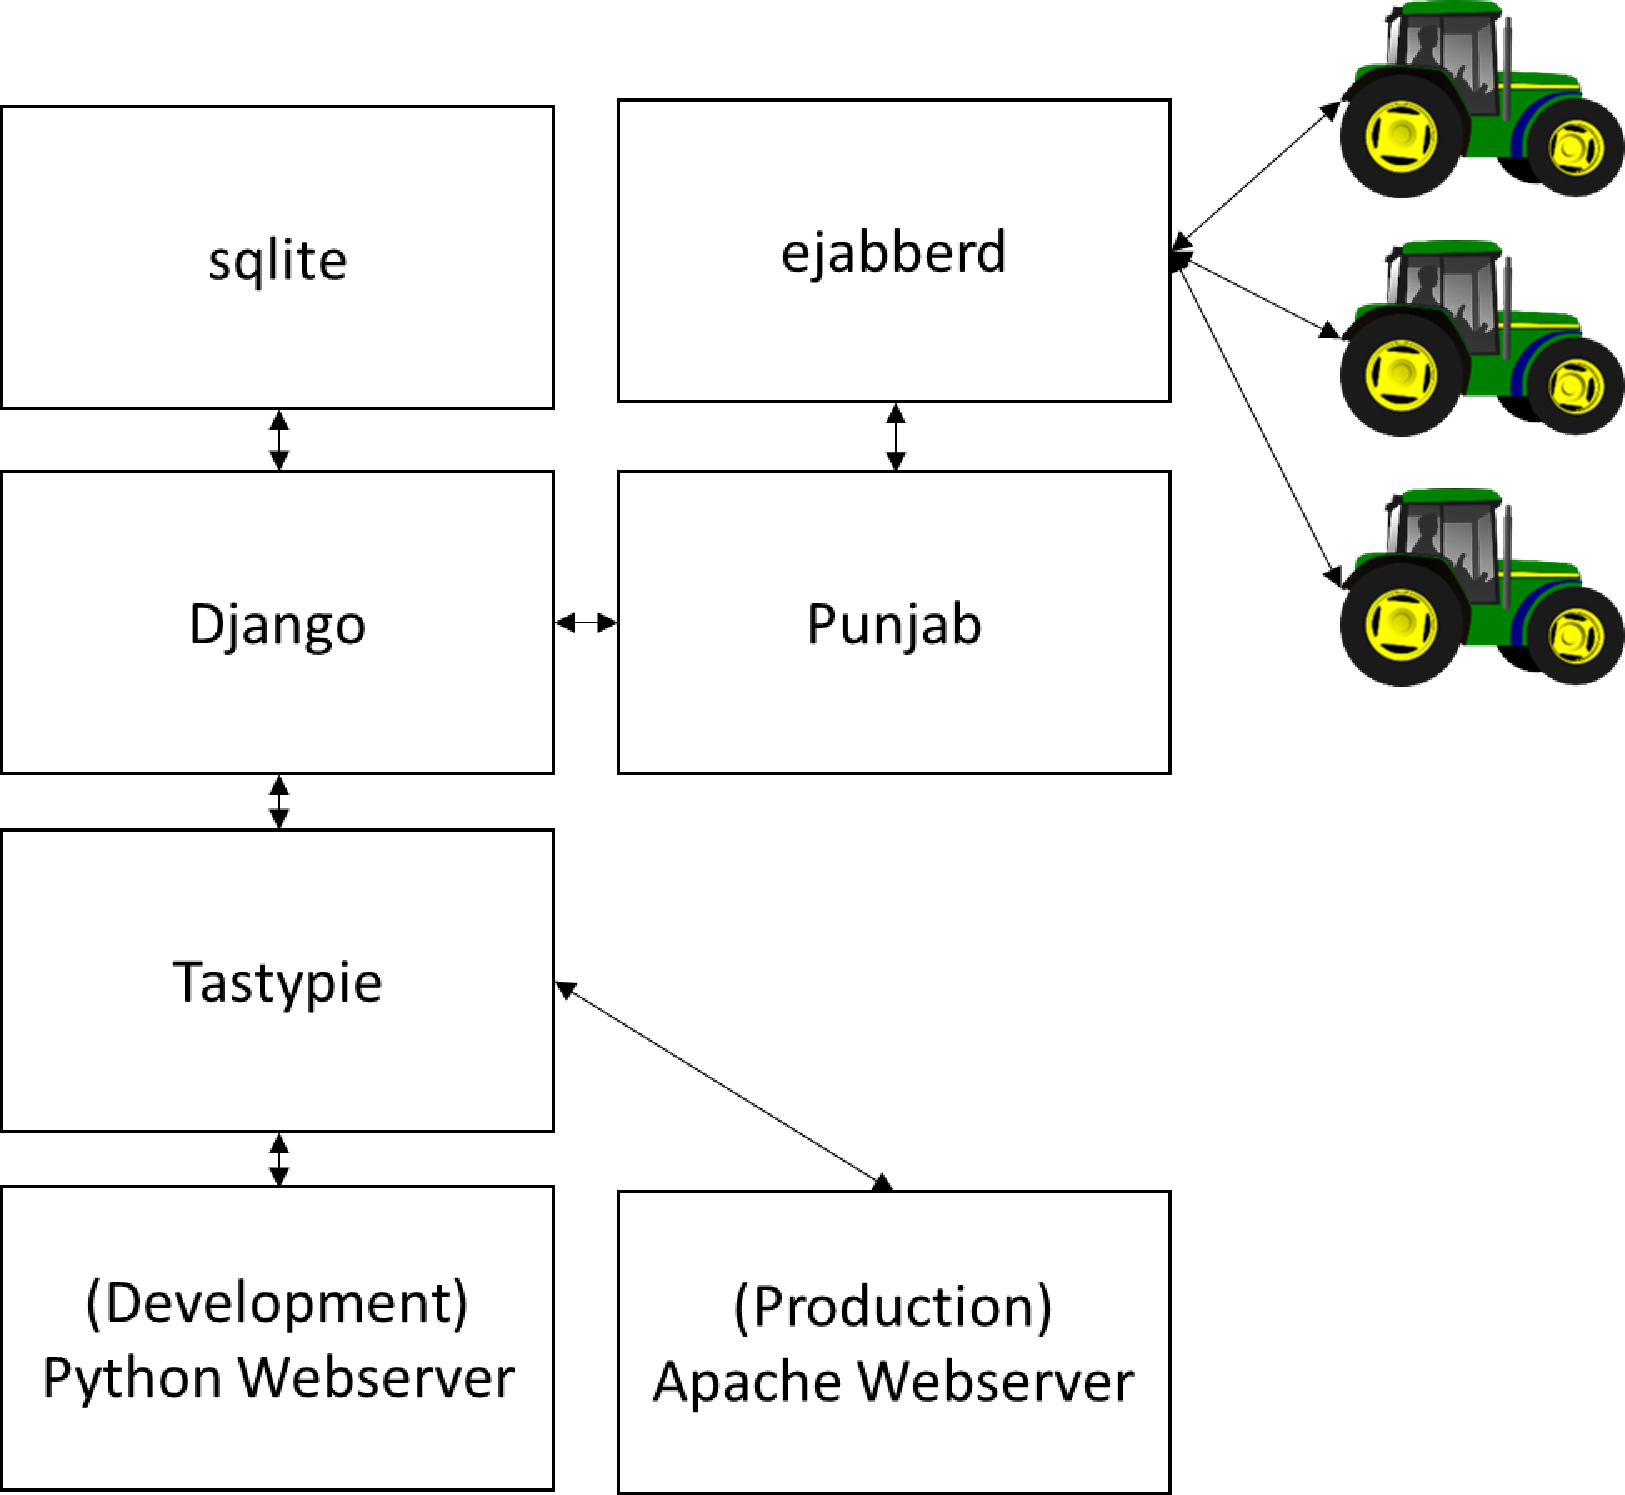
\includegraphics[width=0.4\textwidth]{SoftwareComponentBlockDiagram.pdf}
\caption{Software Component Block Diagram}
\label{fig:softwarecomponents}
\end{figure}

\subsection{Security Model}
RoboTractor deals with two primary security classes: One involving the vehicles
and other assets, and one involving the system components and their communication channels.
Because the project is web-based and uses PKI, numerous attack models have
been created that this project will deal with. Within the class of communication channels,
attacks may be present against the authentication systems of both users and assets. Robotractor \DIFdelbegin \DIFdel{will employ
}\DIFdelend \DIFaddbegin \DIFadd{currently employs
}\DIFaddend advanced two-factor authentication. Usage of TLS and other best common practices will \DIFdelbegin \DIFdel{help }\DIFdelend \DIFaddbegin \DIFadd{be implemented }\DIFaddend to prevent
against replay attacks on the system, and also for establishing a secure session between assets and control.
A dual-encryption scheme has been devised to send encrypted control signals within an encrypted XMPP stanza
to ensure high information assurance. Because this project will utilize PKI, key protection is important. To this end
the RoboTractor project plans to secure keys on assets with a Trusted Platform Module or relevant simulated facsimile.
By making both key-pairs private and secure, RoboTractor provides advanced communication security.
On the other end, the server components must be secured as well using best common practices in server defense, firewall,
patches, updates, etc. Additionally, the RoboTractor system will implement an advanced GPS location reporting system
to provide physical security in case of asset theft. By defending against these attack models, the RoboTractor project
presents the realization of an advanced system for signaling and control with high security. 

\section{Project Description}
Implementation is divided into 2 primary phases (Marked as milestones on the
attached Gantt chart).  The first phase is an integration phase connecting
the various libraries and off the shelf components. It is critical that this
integration does not weaken, but rather strengthens the security properties
provided by each independent component. 

The second phase is the extension of these components to provide command and
control of agricultural vehicles. For schedule mitigation, David and Arun are
scheduled to begin this phase before the framework is assembled. Once the
framework is in place, David and Arun's interface designs may be merged with the
overall system. \DIFdelbegin \subsection{\DIFdel{Task 1 : Development Environment}}
%DIFAUXCMD
\addtocounter{subsection}{-1}%DIFAUXCMD
\DIFdel{The development environment consists of configuring all the tools needed to portably work with the software package. This will involve installing project dependencies, and deployment scripts to allow all members of
the team to work
effectively together.
The complete environment will be stored in git.
}\DIFdelend \DIFaddbegin \DIFadd{As of the creation of this document, all Midterm deliverables have been achieved.
The following tasks have been updated to reflect work currently done, and remaining future work.
}

\subsection{\DIFadd{Task 1 : Development Environment}}
\DIFadd{This task consisted of setting up the development environment for the RoboTractor project. 
A project homepage was provided to us via the ASU virtual lab project. This home page provides
source control in the form of a GIT repo which our project takes advantage of. Additionally, two
virtual machines were provided via the ASU virtual lab project to use as our project servers. Setup of
these servers was automated with the creation of a script in order to download all required software packages.
Remaining work for this task is to enable proper connectivity between the two assigned VM's once all RoboTractor components are operational.
}\DIFaddend \subsection{Task 2: XMPP Implementation}
XMPP Implementation is a configuration task to setup the ejabberd
server and connect it into the HTTP Framework. Once this is in place the XMPP
Clients may start working. \DIFdelbegin \subsection{\DIFdel{Task 3: Demo Tractor}}
%DIFAUXCMD
\addtocounter{subsection}{-1}%DIFAUXCMD
\DIFdel{The Demo tractor is the complementary component to the Frontend UI.
This is the virtual machine, a piece of software which simulates a real tractor , or
agricultural vehicle . 
}\DIFdelend \DIFaddbegin \DIFadd{The XMPP client/server components and interfacing with them is not a midterm deliverable, and is to be finished before final submission.
}\subsection{\DIFadd{Task 3: Demo Tractor}}
\DIFadd{The midterm deliverable for this task was to finalize the design specifications of the tractor simulator. This has been achieved after multiple team discussions, and a barebones
state machine vehicle simulator has been written in python. As more tasks are completed, the simulator is to be updated with its required functionality such as XMPP communication, path processing, and status reporting.
}\DIFaddend \subsection{Task 4: Frontend UI}
The "single-page" web application is the modern design methodology to web apps
today. Leveraging this design architecture the Frontend will query the REST API
to draw the position of all tractors within a Google Map context. \DIFaddbegin \DIFadd{Additionally, 
the frontend user interface is to be highly secure. }\DIFaddend This task has
2 high level sub tasks:
\begin{enumerate}
\item Path generation
\item Map rendering
\end{enumerate}
Path generation is the primary deliverable of this \DIFdelbegin \DIFdel{project}\DIFdelend \DIFaddbegin \DIFadd{task}\DIFaddend . The user shall be
able to input a path for a given tractor to drive. The Tractor will then receive
this path over the REST to XMPP \DIFdelbegin \DIFdel{gateway}\DIFdelend \DIFaddbegin \DIFadd{channel}\DIFaddend .  The UI may then periodically query the
position of the tractor and update it on the Google Map. \DIFaddbegin \DIFadd{Currently, a test-interface has been completed to meet the midterm deliverables, with additional functionality forthcoming.
}\DIFaddend \subsection{Task 5: Server Backend}
The Server Backend is the critical component which \DIFdelbegin \DIFdel{plumbs all the componentstogether}\DIFdelend \DIFaddbegin \DIFadd{connects all components}\DIFaddend .
Extensive knowledge of Django will make this task easier. As it will
require linking multiple components together in a orchestrated fashion. \DIFaddbegin \DIFadd{We have currently setup and tested our server running on Django, and will continue to update as needed over the course of the project.
}\DIFaddend \subsection{Task 6: REST Interface}
The REST interface will server the primary means of interacting with the site.
The Web interface will exist as a "single-page" app \DIFdelbegin \DIFdel{who }\DIFdelend \DIFaddbegin \DIFadd{which }\DIFaddend leverages AJAX
principles over this REST API. \DIFaddbegin \DIFadd{The REST interface is currently functional, and will be updated to interface further with the frontend interface and backend components as they are completed.
}\DIFaddend \subsection{Project Task Allocation}

From the tasks outlined in section III, the breakdown of work \DIFdelbegin \DIFdel{will be }\DIFdelend \DIFaddbegin \DIFadd{is }\DIFaddend as follows:
Jeremy Wright \DIFdelbegin \DIFdel{will work on configuring }\DIFdelend \DIFaddbegin \DIFadd{has configured }\DIFaddend the development environments and the REST Interface. \DIFdelbegin \DIFdel{He will operate }\DIFdelend \DIFaddbegin \DIFadd{Jeremy is also looking into modelling trust zones which would allow us to simulate trusted hardware in actual vehicles.
He is operating }\DIFaddend as the project lead due to his experience in Python-based Web Applications.
Arun Balaji Buduru \DIFdelbegin \DIFdel{will work }\DIFdelend \DIFaddbegin \DIFadd{is working }\DIFaddend on the Server Backend and Frontend UI components. \DIFdelbegin \DIFdel{David Lucero will work }\DIFdelend \DIFaddbegin \DIFadd{He has completed a front-end test interface and is continuing to update it to achieve all required functionality.
David Lucero is working }\DIFaddend primarily on the \DIFdelbegin \DIFdel{Demo Tractor }\DIFdelend \DIFaddbegin \DIFadd{Tractor simulation }\DIFaddend agents and also XMPP implementation. \DIFaddbegin \DIFadd{A barebones tractor simulation has been completed and will be continuously updated as the project progresses.
}\DIFaddend Each group member \DIFdelbegin \DIFdel{will have }\DIFdelend \DIFaddbegin \DIFadd{has }\DIFaddend approximately 30\% workload of the project with the remaining
10\% shared due to the interconnected nature of all components. A detailed task breakdown
can be seen in the attached Timeline.

\subsection{Deliverables}

Midterm Deliverables:
\begin{enumerate}
\item Functioning REST Interface \DIFaddbegin \DIFadd{(completed)
}\DIFaddend \item Front-end Test Interface \DIFaddbegin \DIFadd{(completed, with additional two factor-authentication)
}\DIFaddend \item API documentation for using the REST interface as an external service. \DIFaddbegin \DIFadd{(moved to final deliverable)
}\DIFaddend \item API documentation for using the XMPP interface to act as a vehicle. \DIFaddbegin \DIFadd{(moved to final deliverable)
}\DIFaddend \item Finalized Design of Vehicle simulator \DIFaddbegin \DIFadd{(completed, with additional python test implementation)
}\DIFaddend \item Interim Progress Report \DIFaddbegin \DIFadd{(completed)
}\DIFaddend \item Updated Project Schedule \DIFaddbegin \DIFadd{(completed)
}\item \DIFadd{Interim Project Powerpoint Presentation (completed)
}\DIFaddend \end{enumerate}

Final Deliverables:
\begin{enumerate}
\item Finalized back-end \DIFdelbegin \DIFdel{configuration
}\DIFdelend \DIFaddbegin \DIFadd{server configuration including easy installation script(s)
}\DIFaddend \item \DIFdelbegin \DIFdel{Administration panel for configuring vehicles.
}%DIFDELCMD < \item %%%
\DIFdel{Finalized }\DIFdelend \DIFaddbegin \DIFadd{Completed, secure }\DIFaddend front-end interface \DIFaddbegin \DIFadd{including two-factor auth and SSL/TLS.
}\DIFaddend \item Vehicle Simulator with working component interfaces \DIFaddbegin \DIFadd{and simulated trust zone functionality
}\DIFaddend \item Final Project Report
\DIFaddbegin \item \DIFadd{Final Project Powerpoint Presentation
}\item \DIFadd{User-guide covering front-end interface, and including API documentation for REST and XMPP interfaces 
}\DIFaddend \end{enumerate}


\subsection{Project Timeline}
The attached project timeline (generated from Microsoft Project) describes the
overall tasks of the project.
\section{Risk Management of the project}
Several potential issues have been identified that may pose risk to successful
completion of this project. These risks have been identified in Table
\ref{tab:riskmanagement}. Along with the description, ratings have been assigned
to each risk identified, and potential mitigation strategies are described.

\section{Conclusion}
In this proposal we intend to build a remote control system leveraging existing
internet technologies \DIFaddbegin \DIFadd{such as }\DIFaddend XMPP and REST. Future work based on this approach may
include asset management for corporate farm management.

\printbibliography
\clearpage
\begin{landscape}
\begin{table}%[!t]
%\renewcommand{\arraystretch}{1.3}
\caption{Risk Management}
\label{tab:riskmanagement}
\centering
\begin{tabular}{c||c||p{2in}||p{2in}}
\hline
\bfseries Risk Description & \bfseries Risk of Failure & \bfseries Consequence of Failure & \bfseries Mitigation Strategy\\
\hline\hline
Connections between components must be secure
& Low
& Product would still function, but would lack security – information assurance will suffer
& Plan to include security on component connections ahead of time. Follow best practices (SSL/TLS)\\
\hline
Evaluation of Project depends on proper vehicle agents
& Medium
& System is unable to be tested if vehicle agents are inoperable or incorrect
& Vehicle agents will be designed first to ensure compatibility with all other components. Thorough review and testing of component to ensure proper functionality\\
\hline
Improper configuration of components
& Medium
& Components do not communicate properly with each other. System functionality is void
& Thorough reviews and testing of components to ensure proper functionality and communication\\
\hline
Incorrect PKI implementation and/or configuration
& Medium
& Puts all identified security domains at risk. PKI used becomes useless. System becomes vulnerable to outside attacks i.e. MITM
& Follow best practices and standards. No re-invention of the wheel\\
\hline
Service Uptime (web reliably)
& High
& Product is unusable if network connections are not operable
& Redundancy. Cloud hosting to alleviate hardware reliance\\
\hline
\end{tabular}
\end{table}
\end{landscape}
\end{document}


